\documentclass[conference]{IEEEtran}
\IEEEoverridecommandlockouts

\usepackage{cite}
\usepackage{amsmath,amssymb,amsfonts}
\usepackage{graphicx}
\usepackage{textcomp}
\usepackage{xcolor}
\usepackage{array}
\usepackage{booktabs}
\usepackage{url}
\usepackage{tikz}
\usepackage{float}
\usepackage{tikz}
\usepackage{pgfplots}
\pgfplotsset{compat=1.18}
\usetikzlibrary{shapes.geometric, arrows.meta, positioning, fit, calc}

\begin{document}

\title{MediaPipe-Based Hand Gesture Recognition and Tracking for Real-Time Virtual Canvas Interaction and Digital Drawing}

\author{
\IEEEauthorblockN{Dr. Anita Harsoor, Hisham Khuram, Md Ahmed Raza Sofi, Mohammad Abdul Maaz Hanan}
\IEEEauthorblockA{Department of Computer Science and Engineering\\
P.D.A. College of Engineering\\
Kalaburagi, India\\
anitaharsoor@pdaengg.com, 3pd23cs050@pdaengg.com, 3pd23cs065@pdaengg.com, 3pd23cs070@pdaengg.com}
}

\maketitle

\begin{abstract}
Touchless human–computer interaction enables direct control of digital content through physical movement. This paper presents AirSketch, a real-time gesture-based virtual drawing system developed using Python, OpenCV, MediaPipe, and NumPy. A standard webcam captures hand movements, while MediaPipe detects hand landmarks and uses the index fingertip as the interaction point. A distance-based pinch gesture activates drawing and shape creation, while a five-sample moving average reduces cursor jitter. The system supports freehand drawing, erasing, geometric shapes, color selection, brush-size control, and canvas clearing. AirSketch uses a lightweight, deterministic approach without requiring depth cameras, gloves, or trained gesture classifiers. The paper discusses its architecture, interaction model, rendering process, implementation, and functional evaluation, along with limitations such as sensitivity to lighting and camera quality, single-hand operation, and limited gesture vocabulary.
\end{abstract}

\begin{IEEEkeywords}
hand gesture recognition, human--computer interaction, MediaPipe, OpenCV, virtual drawing, touchless interface, hand landmarks, computer vision
\end{IEEEkeywords}

\section{Introduction}

Human--computer interaction has increasingly incorporated natural input modalities that reduce dependence on traditional devices such as keyboards, mice, styluses, and touchscreens. Hand gestures are particularly useful because they can express pointing, selection, movement, and manipulation without requiring a physical controller. Research in this area includes skeleton-based gesture recognition, air-writing, virtual painting, assistive interfaces, sign-language recognition, and sensor-based interaction.

The sensing modality has a substantial influence on the design of a gesture-controlled system. AO-Finger introduced a wrist-worn acoustic-optic sensing system for fine-grained finger gesture recognition by combining acoustic and optical measurements and evaluating gestures including Flick, None, Pinch, and Tap \cite{ao_finger}. Its results demonstrate the usefulness of specialized sensing hardware for detailed finger interaction. In contrast, OMG-Bench addresses online micro hand gestures using skeleton-based representations and provides a benchmark for evaluating subtle hand movements \cite{omgbench}. Air-writing research has also explored webcam-based fingertip tracking and handwriting recognition using OpenCV and MediaPipe \cite{airwriting}. Air Canvas Hand Tracking demonstrates the use of camera-based hand tracking for virtual drawing and interaction \cite{swathi}. A multimodal depth-aware system by Mahmud et al. investigates dynamic gesture recognition using depth and skeletal information, illustrating the potential of richer multimodal inputs \cite{mahmud}.

Other computer-vision approaches have examined feature extraction and machine-learning methods for hand gesture recognition. Sharma et al. investigate image-processing and feature-extraction techniques for gesture classification using conventional machine-learning models \cite{sharma}. Qi et al. provide a review of computer-vision-based hand gesture recognition for human--robot interaction and discuss the broader challenges associated with gesture perception and interaction \cite{qi2024}. Morajkar et al. combine hand gesture and voice interaction for computer control, demonstrating the application of gesture recognition to assistive interfaces \cite{morajkar}. Anithadevi et al. combine MediaPipe with an LSTM-based architecture for dynamic sign-language recognition, demonstrating how landmark sequences can be used as input to temporal learning models \cite{anithadevi2025}. Software-oriented research also highlights the importance of reliability in machine-learning systems implemented using JavaScript-based frameworks \cite{quan}.

Virtual drawing systems provide a more application-specific use case for hand tracking. Vasavi et al. present a virtual painting system based on hand gestures and MediaPipe, demonstrating that fingertip tracking can be used to replace physical drawing input \cite{vasavi}. Dynamic gesture recognition using spatiotemporal representations has also been explored for LIBRAS gesture recognition, where MediaPipe landmarks are arranged into temporal representations and classified using a convolutional neural network \cite{moreira2026}. AirSketch: Generative Motion to Sketch addresses a different problem in which noisy hand-motion representations are transformed into visually coherent sketches using a learned generative approach \cite{generative_airsketch}. A gesture-based Virtual Write and Clear application similarly uses MediaPipe and OpenCV to provide drawing, color selection, and erasing through hand interaction \cite{virtualwrite}. Virtual Hand Gesture Painting investigates a MediaPipe and OpenCV-based virtual painting interface in which hand movements are converted into digital drawing operations \cite{virtualpainting}.

Although these systems demonstrate the feasibility of gesture-controlled interaction, their objectives, sensing modalities, datasets, gesture vocabularies, and evaluation protocols differ. AirSketch focuses on a lightweight application-level interaction model in which a standard RGB webcam supplies hand landmarks and deterministic geometric rules convert those landmarks into drawing commands. Rather than training a new gesture classifier, AirSketch uses the relative distance between the index and middle fingertips to determine a pinch state.

The objective is therefore not to propose a new hand-tracking model or claim superiority over existing gesture-recognition systems. Instead, the objective is to demonstrate how established hand-landmark detection can be integrated with simple geometric interaction rules to create a practical and interpretable virtual drawing system.

\section{System Design and Methodology}

\subsection{Design Requirements}
The system was designed around five functional requirements. First, interaction should be possible using a conventional webcam without a wearable device. Second, the system should operate continuously on a live video stream rather than on pre-recorded images. Third, the user should be able to draw both freehand strokes and geometric primitives. Fourth, the interaction mechanism should provide a clear distinction between cursor movement and an intentional drawing action. Finally, the interface should expose essential controls without requiring keyboard-driven tool selection during normal operation.

These requirements lead to a pipeline in which perception, interaction interpretation, drawing state, and display are separated conceptually. The webcam provides the input frame. MediaPipe estimates hand landmarks. A landmark-processing layer extracts the relevant fingertip coordinates and computes the activation state. The virtual-painter layer then interprets the state according to the selected tool and updates either the persistent canvas or a temporary preview. The UI layer renders the toolbar and responds to pointing interactions in the toolbar region.

\subsection{Overall Processing Workflow}

As illustrated in Fig.~\ref{fig:architecture}, AirSketch follows a continuous frame-based processing workflow. The process begins with the acquisition of live video frames from the webcam at a resolution of 1280 $\times$ 720 pixels. Each frame undergoes horizontal flipping and preprocessing before being passed to MediaPipe Hands, which detects the hand and identifies its 21 landmarks.

The system first checks whether a hand has been detected. If no hand is detected, hand interaction processing is skipped, and the existing drawing canvas is retained. Otherwise, the index and middle fingertip coordinates are extracted. The index fingertip coordinates are then smoothed using a five-frame moving average to reduce unwanted fluctuations and provide more stable pointer movement.

Following coordinate processing, the system processes toolbar selections and updates the currently selected control. It then evaluates the distance between the index and middle fingertips to determine whether a pinch gesture is active. The pinch state is determined using a fixed threshold of 70 pixels. If a pinch is detected, the selected drawing operation is performed. This may involve freehand drawing using the brush, removing existing content using the eraser, or generating a temporary preview for a geometric shape.

If no active pinch is detected, the system proceeds to finalize the drawing action, committing a geometric shape when required. The resulting interaction state is then passed to the canvas compositing stage. During this stage, the drawing canvas is combined with the original camera frame to produce the final visual output. The toolbar and fingertip cursor are subsequently rendered onto the composite image, which is displayed to the user. The process then continues with the detection of subsequent video frames, enabling continuous real-time interaction.

\subsection{Video Acquisition and Preprocessing}
The main application opens the default camera through OpenCV's `VideoCapture(0)` interface. The requested capture dimensions are 1280 by 720 pixels. Each frame is horizontally flipped before processing, producing a mirror-like interaction view that corresponds more naturally to the user's physical movement. The frame is then passed to the virtual painter, which orchestrates hand tracking, interaction logic, drawing, and final compositing.

The use of a fixed 1280 by 720 working space simplifies coordinate mapping because the landmark coordinates are converted directly into pixel positions using the same dimensions. MediaPipe itself reports normalized image coordinates, with $x$ and $y$ expressed relative to image width and height \cite{mediapipe_docs}. The conversion used by the current implementation is therefore
\begin{equation}
 x_p = \lfloor 1280x_n \rfloor, \qquad y_p = \lfloor 720y_n \rfloor,
\end{equation}
where $(x_n,y_n)$ are the normalized landmark coordinates and $(x_p,y_p)$ are pixel coordinates in the application workspace.

\begin{figure*}[!t]
    \centering
    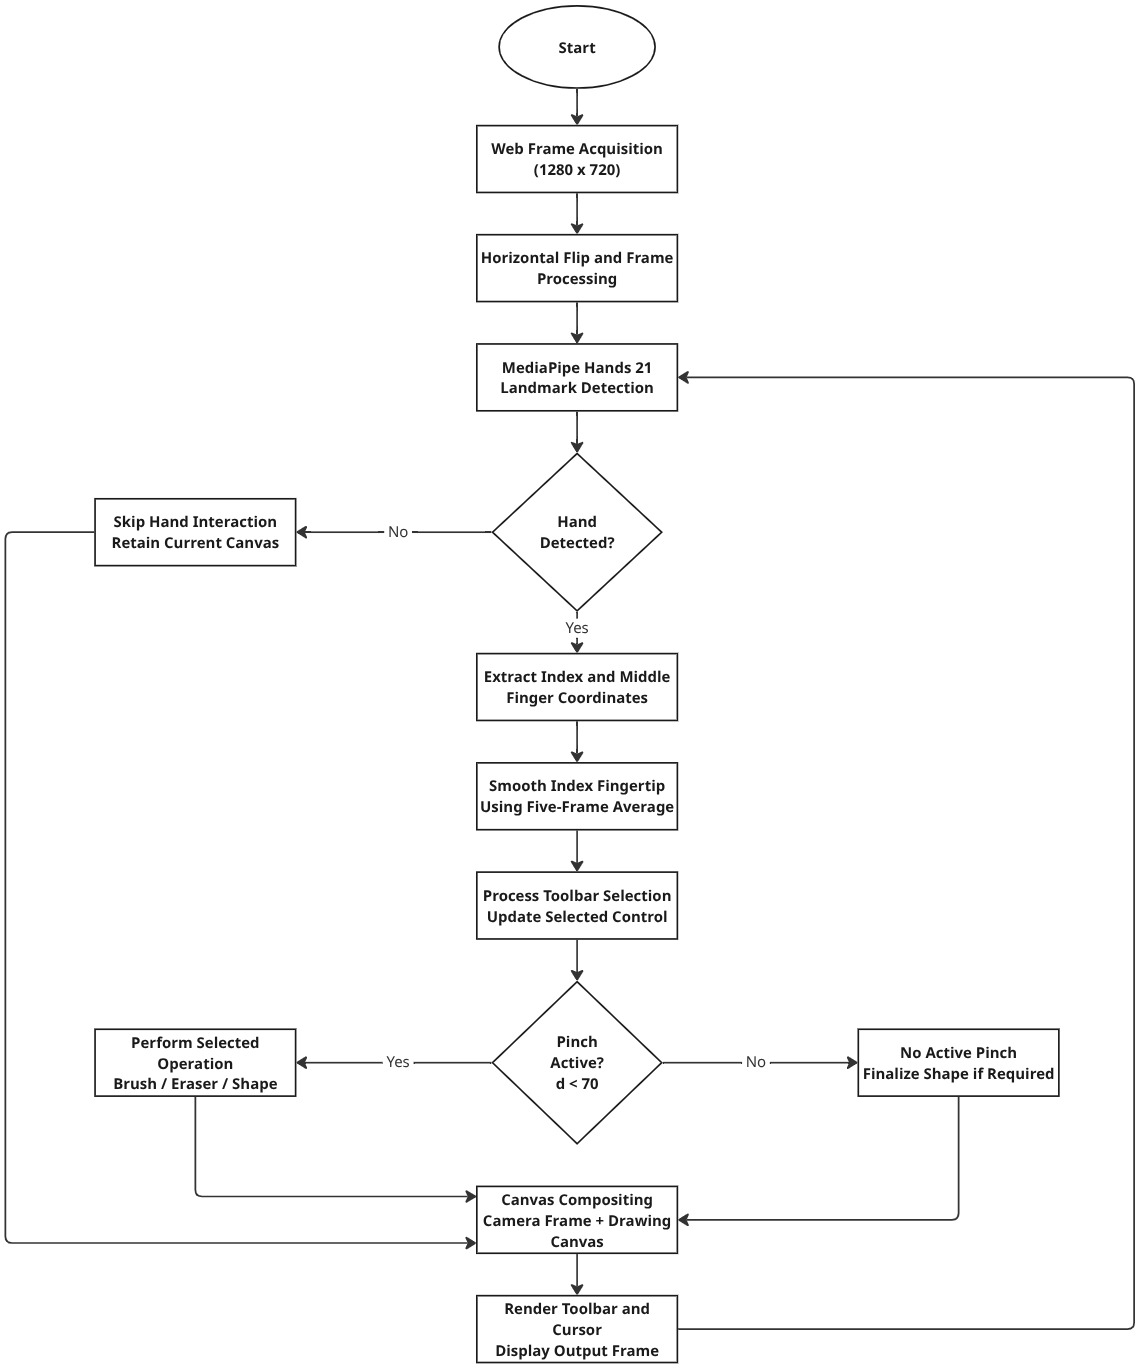
\includegraphics[
        width=\textwidth,
        height=0.73\textheight,
        keepaspectratio
    ]{airsketch_flowchart.jpg}
    \caption{Flowchart illustrating the overall processing
    and interaction workflow of the AirSketch system.}
    \label{fig:architecture}
\end{figure*}

\subsection{Hand Landmark Detection}
AirSketch uses the Python MediaPipe Hands solution with `max\_num\_hands=1`, a minimum detection confidence of 0.75, and a minimum tracking confidence of 0.70. MediaPipe Hands produces 21 landmarks representing the hand skeleton \cite{vasavi}. The current system does not invoke a separate gesture-classification model. Instead, it consumes the landmark coordinates directly.

Two landmarks are central to the interaction model. Landmark 8 corresponds to the index-finger tip, and landmark 12 corresponds to the middle-finger tip \cite{vasavi}. The index tip is used as the virtual pointer position. The distance between the two fingertips is used to determine whether the user is making an active pinch. This choice provides a simple binary interaction state while retaining continuous two-dimensional fingertip motion for drawing.

\subsection{Pinch-Based Interaction Model}
For every detected frame, the Euclidean distance between the index and middle fingertips is computed as
\begin{equation}
 d = \sqrt{(x_{12}-x_8)^2 + (y_{12}-y_8)^2}.
\end{equation}
The current implementation declares the pinch state active when
\begin{equation}
 P =
 \begin{cases}
 1, & d < 70,\\
 0, & d \geq 70.
 \end{cases}
\end{equation}
The threshold is expressed in pixels in the 1280 by 720 processing space. This deterministic rule avoids an additional classification model and makes the activation condition directly interpretable.

When the pinch is active and the hand is outside the toolbar region, the system enters a drawing state. The first active frame initializes the starting coordinates. Subsequent active frames either extend a freehand stroke or update a temporary preview for a geometric shape. When the pinch is released, geometric shapes are committed to the persistent canvas. This press--move--release model is analogous to click-and-drag interaction, but the activation event is generated by the hand rather than a mouse button.

\subsection{Fingertip Smoothing}
Raw landmark coordinates can exhibit small frame-to-frame fluctuations even when the hand is approximately stationary. Such fluctuations are undesirable for freehand drawing because they appear as unintended irregularities. AirSketch therefore stores the five most recent index-fingertip coordinates in a deque and calculates their arithmetic mean. For a window containing $N$ samples, the smoothed point is
\begin{equation}
 \bar{x}_t = \frac{1}{N}\sum_{i=0}^{N-1}x_{t-i}, \qquad
 \bar{y}_t = \frac{1}{N}\sum_{i=0}^{N-1}y_{t-i},
\end{equation}
with $N\leq5$ during startup and $N=5$ after the buffer is filled. The resulting point is rounded to an integer pixel coordinate before being used by the drawing engine. The filter is intentionally simple: it requires negligible additional computation and provides a predictable smoothing effect, although it introduces a small temporal lag compared with using the raw coordinate directly.

\subsection{Drawing State and Tool Operation}
The persistent drawing surface is a 720 by 1280 three-channel NumPy array initialized to black. A second array, `temp\_canvas`, is used for transient previews. The distinction is important for shape creation. If a user begins a rectangle, circle, line, filled rectangle, or filled circle, the system keeps the original canvas unchanged while the current pointer position is used to render a preview. Once the pinch is released, the selected primitive is drawn onto the persistent canvas.

For brush operation, consecutive fingertip positions are connected using OpenCV's line primitive. The previous coordinate is stored in `prev\_x` and `prev\_y`; the current coordinate becomes the endpoint of the next segment. This creates a continuous polyline as the hand moves. The eraser uses the same trajectory mechanism but removes previously rendered content from the canvas representation.

Geometric tools use OpenCV primitives directly. A rectangle is specified by the initial and current fingertip positions. A line uses the same pair as its endpoints. For circles, the initial position serves as the center and the Euclidean distance to the current position determines the radius:
\begin{equation}
 r = \left\lfloor\sqrt{(x_2-x_1)^2+(y_2-y_1)^2}\right\rfloor.
\end{equation}
Both outline and filled versions of rectangles and circles are available. The brush thickness is shared across drawing primitives and can take one of ten values from 5 to 50 pixels in increments of 5 pixels.

\subsection{User Interface and Control Layer}
The interface is drawn directly onto the camera frame using OpenCV. A toolbar occupies the upper part of the 1280 by 720 display, with a configured height of 82 pixels. The toolbar contains the AirSketch title, twelve color choices, eight tool buttons, and brush-size controls. Tool icons are loaded from PNG assets stored inside the project repository.

The eight available tools are brush, eraser, rectangle, circle, line, filled rectangle, filled circle, and clear canvas. Selecting a color changes the current drawing color. The brush-size section provides decrement and increment buttons and constrains the selected size to the predefined ten-value list. The clear operation replaces the persistent canvas with a new zero-valued image and resets relevant drawing state.

A hand whose smoothed fingertip lies within the toolbar region is treated as a UI interaction rather than a drawing action. The interface uses a 0.3-second debounce interval between UI interactions. This prevents repeated selections when the fingertip remains over the same button across multiple frames. The separation between toolbar and drawing region therefore forms an additional state constraint in the interaction model.

\subsection{Canvas Compositing and Display}
The drawing canvas is not displayed as a separate opaque window. Instead, the application extracts a binary mask from the current drawing image. Pixels above a grayscale threshold of 5 are treated as foreground, while the remaining pixels allow the original camera image to remain visible. The masked camera frame and masked drawing canvas are then added to produce the final composite image.

This approach creates the visual effect of drawing in the physical camera view. The fingertip cursor is rendered after the toolbar and canvas compositing, ensuring that the current interaction point remains visible above other display elements. For the eraser, the cursor preview is rendered using black rather than the current color.

\section{Implementation}

\subsection{Software Stack}
The current project is intentionally small. Its declared Python dependencies are MediaPipe 0.10.21, OpenCV 4.10.0.84, and NumPy 1.26.4 \cite{repo}. MediaPipe provides hand perception, OpenCV provides camera access, image manipulation, rendering primitives, and the desktop display loop, while NumPy provides the image-array representation used for the persistent and temporary canvases. No React, TypeScript, TensorFlow.js, Vite, Tailwind CSS, or browser canvas framework is present in the current implementation.

The source code is organized into three principal Python modules. `main.py` manages camera acquisition and the application loop. `hand\_tracker.py` encapsulates MediaPipe initialization, landmark processing, pinch detection, and fingertip smoothing. `virtual\_painter.py` maintains canvas state, tools, colors, brush size, drawing states, and frame processing. `ui.py` is responsible for toolbar rendering, icon loading, and pointer-based UI interactions. This modular separation keeps perception, drawing behavior, and presentation logic relatively independent.

\subsection{Hand Tracker Module}
The hand tracker converts each BGR frame into RGB before passing it to MediaPipe. If no hand is detected, it returns `None`, allowing the rest of the pipeline to retain the existing canvas while skipping interaction updates. When a hand is detected, MediaPipe's hand connections are rendered on the frame for visual feedback. The implementation then extracts landmarks 8 and 12 and converts their normalized coordinates to pixels.

The tracker maintains a fixed-length deque with five entries. Every valid index-fingertip position is appended, and the arithmetic mean of the available positions is returned. Because the deque is updated only when a hand is present, the filter naturally resets its effective window when tracking resumes after an absence. The current code does not perform temporal classification, velocity estimation, Kalman filtering, or adaptive thresholding.

\subsection{Virtual Painter Module}
The `VirtualPainter` object initializes the persistent canvas and temporary canvas, sets the default color and brush size, defines the available tools, and creates the hand tracker and UI objects. It also maintains the interaction state variables `drawing`, `prev\_x`, `prev\_y`, `start\_x`, and `start\_y`.

The `process\_frame` method is the central orchestration function. It first copies the persistent canvas into the temporary canvas. It then obtains hand data. If the hand is detected above the toolbar boundary, UI interaction handling takes precedence. If the hand is in the drawing region and the pinch is active, the system either starts a new interaction, extends a brush/eraser stroke, or renders a geometric preview. On pinch release, geometric tools are committed to the persistent canvas. Finally, the selected display surface is composited with the camera frame and passed to the UI renderer.


\begin{table}[t]
\caption{AirSketch Interaction Mapping}
\label{tab:interaction}
\centering
\scriptsize
\begin{tabular}{p{1.45cm}p{1.65cm}p{2.55cm}}
\toprule
\textbf{Input} & \textbf{Condition} & \textbf{System action}\\
\midrule
Index fingertip & Hand detected & Virtual pointer position\\
Index + middle tips & Distance $<70$ px & Active pinch/drawing state\\
Pinch + brush & Continuous movement & Freehand stroke\\
Pinch + eraser & Continuous movement & Blank stroke for erasing\\
Pinch + shape tool & Movement & Temporary geometric preview\\
Pinch release + shape & End of interaction & Commit shape to canvas\\
Pointer in toolbar & $y<90$ & UI interaction mode\\
Pointer on color & Within selection radius & Change drawing color\\
Pointer on tool & Within button bounds & Change active tool\\
Pointer on size control & Button bounds & Increase/decrease thickness\\
Pointer on clear & Clear button bounds & Reset persistent canvas\\
\bottomrule
\end{tabular}
\end{table}

\subsection{User Interface Module}
The UI module creates the toolbar using OpenCV drawing functions. It loads the tool icons from the repository's `assets/icons` directory and supports alpha compositing for PNG images. Color selection is performed by testing the distance from the pointer to each color-circle center. Tool selection is performed by checking whether the pointer lies inside a tool button's rectangular bounds. Brush-size selection uses separate rectangular controls for decrement and increment operations.

The interface uses a 0.3-second debounce time for all UI interactions. This is a practical mechanism for reducing repeated selections caused by the high temporal sampling rate of the video stream. Importantly, the debounce applies to UI selection and not to the continuous drawing path itself, so it does not intentionally suppress ordinary brush motion.

\subsection{Interaction Mapping}
Table~\ref{tab:interaction} summarizes the current interaction model. The table distinguishes between the physical input, the interpretation performed by the software, and the resulting application behavior.

\section{Results}

\subsection{Visual Output Evaluation}

Representative outputs of the AirSketch system are shown in Fig.~\ref{fig:airsketch_outputs}. The first output demonstrates the main drawing interface during operation. The webcam captures the user's hand while MediaPipe landmarks are displayed over the detected hand. The index fingertip is used as the primary interaction point for controlling drawing operations.

The output demonstrates multiple drawing capabilities within a single interaction session. Freehand strokes, a straight line, and geometric shapes are visible directly over the live video feed. The interface also provides controls for brush, eraser, line, rectangle, circle, filled rectangle, filled circle, color selection, canvas clearing, and brush-size adjustment. In the shown example, the circle tool is highlighted, demonstrating that the hand-based pointer can also be used to interact with the toolbar.

The second output demonstrates continued hand-based interaction with content already drawn on the video feed. The detected hand landmarks remain visible while the fingertip is positioned over the displayed drawing. This demonstrates that the landmark-tracking mechanism remains active while interacting with previously created visual content.

The displayed outputs provide functional evidence that the implemented perception and interaction pipeline can translate hand movement into drawing operations using a conventional RGB webcam. Unlike a separate black or blank drawing canvas, the current implementation renders the drawing content directly onto the live video frame, allowing the user to interact with the virtual drawing while simultaneously viewing the camera feed. However, these images represent representative functional demonstrations rather than quantitative measurements of recognition accuracy, latency, or robustness.

\begin{figure}[!t]
    \centering

    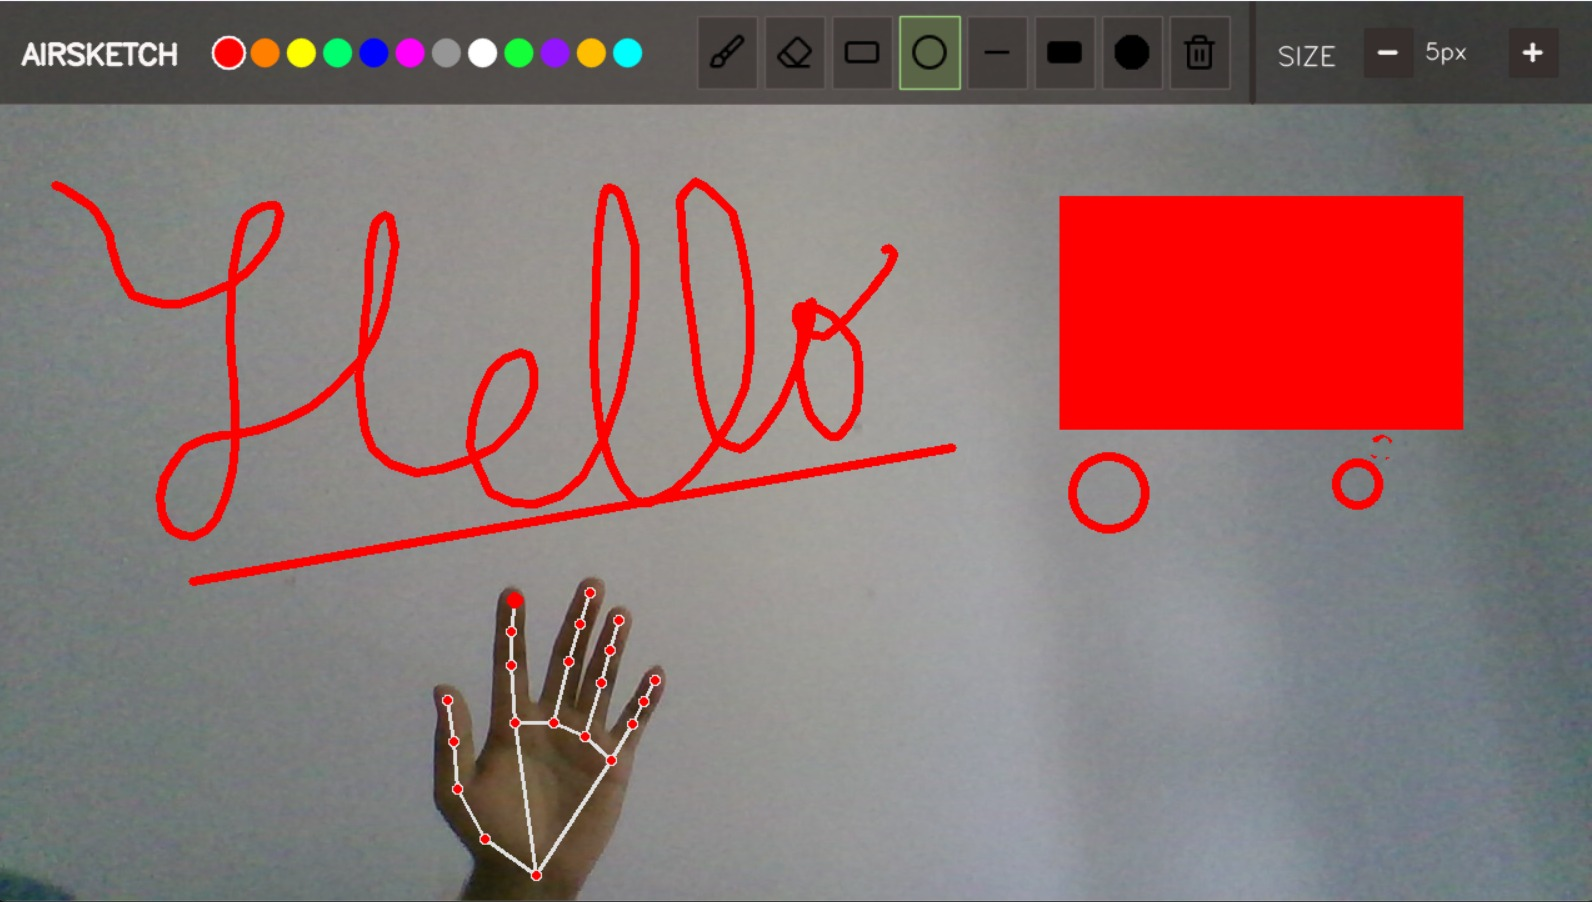
\includegraphics[width=\columnwidth]{drawing_output.jpeg}
    
    \centerline{\footnotesize (a) Drawing and shape creation}
    
    \vspace{0.3cm}
    
    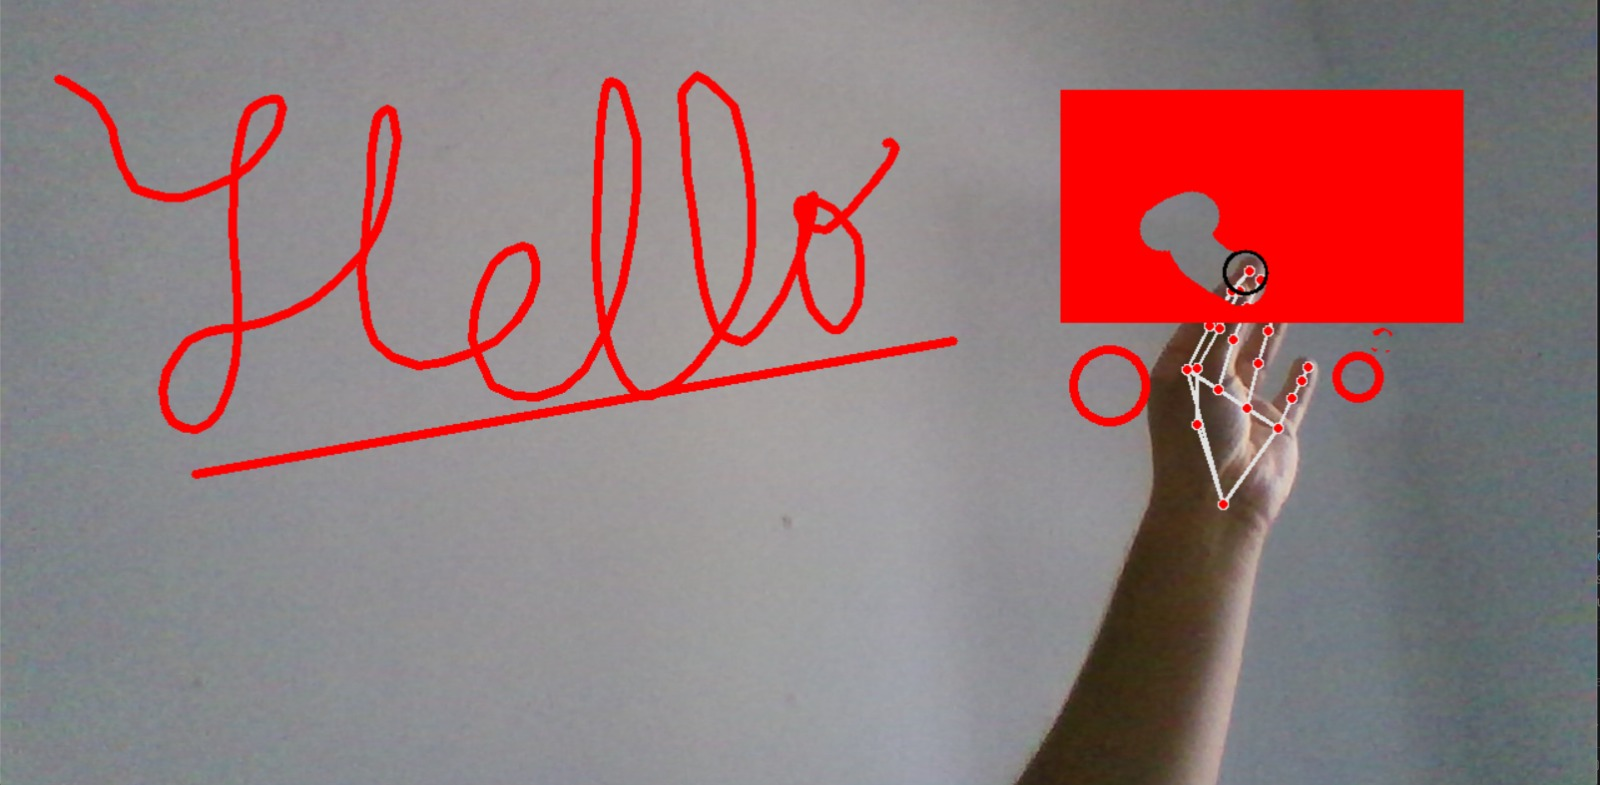
\includegraphics[width=\columnwidth]{interaction_output.jpeg}
    
    \centerline{\footnotesize (b) Hand-based canvas interaction}

    \caption{Representative AirSketch outputs demonstrating (a) freehand drawing, line and geometric shape creation with hand landmark tracking, and (b) hand-based interaction with previously drawn content directly over the live video feed.}
    \label{fig:airsketch_outputs}
\end{figure}

\subsection{Observed Interaction Characteristics}

The application performs hand tracking and drawing within the same frame-processing loop, allowing continuous interaction. The five-sample moving-average filter reduces small coordinate variations before they reach the drawing functions. For freehand tools, the drawing path is rendered incrementally using consecutive fingertip positions. For geometric tools, a temporary frame is used to preview the shape during interaction before the final geometry is committed to the displayed drawing.

The interaction model also provides a clear separation between pointer movement and activation. A user can move the fingertip without producing a new stroke when the pinch is inactive. When the pinch becomes active, the same fingertip trajectory becomes meaningful drawing input. This state-based behavior allows the user to control when a drawing operation begins and ends without requiring a physical pointing device.

The toolbar provides another level of interaction separation. When the smoothed fingertip enters the configured toolbar region, its position can be interpreted as a tool or color-selection command rather than as drawing input. The implemented debounce mechanism reduces repeated UI changes when the pointer remains over a control.

The screenshots also demonstrate that the hand-landmark visualization provides immediate feedback about the detected hand position. The user can observe the tracked hand and fingertip while drawing directly over the camera feed, providing a visual connection between physical movement and the resulting digital content.

\subsection{Discussion}

The evaluation report generated by the AirSketch implementation is summarized in Table~\ref{tab:evaluation_report}. The evaluation was performed on 293 samples to assess the reliability of the pinch-detection mechanism.

\begin{table}[!htbp]
\centering
\caption{AirSketch Pinch-Detection Evaluation Report}
\label{tab:evaluation_report}

\setlength{\tabcolsep}{8pt}
\renewcommand{\arraystretch}{1.35}

\begin{tabular}{lcc}
\hline
\multicolumn{3}{c}{\textbf{Confusion Matrix}} \\
\hline
\textbf{Actual / Predicted} & \textbf{No Pinch} & \textbf{Pinch} \\
\hline
No Pinch & 137 & 0 \\
Pinch    & 8   & 148 \\
\hline
\end{tabular}

\vspace{0.35cm}

\begin{tabular}{lc}
\hline
\multicolumn{2}{c}{\textbf{Evaluation Metrics}} \\
\hline
\textbf{Metric} & \textbf{Value} \\
\hline
Samples   & 293 \\
Accuracy  & 97.27\% \\
Precision & 100.00\% \\
Recall    & 94.87\% \\
F1-score  & 97.37\% \\
FPR       & 0.00\% \\
FNR       & 5.13\% \\
\hline
\end{tabular}
\end{table}


\subsubsection{Confusion Matrix and Evaluation Metrics}

The performance of the AirSketch pinch detection system
was evaluated using a binary classification approach,
where pinch and no-pinch states were considered the
positive and negative classes, respectively.

The confusion matrix was constructed by comparing the
actual gesture state (ground truth) with the predicted
gesture state generated by the system. Four outcomes
were considered: True Positive (TP), True Negative (TN),
False Positive (FP), and False Negative (FN).

The evaluation metrics were calculated using the
following equations:

\begin{flalign}
&\begin{aligned}
\text{Accuracy} &= \frac{TP+TN}{TP+TN+FP+FN} \\[6pt]
&= \frac{148+137}{148+137+0+8} \\[6pt]
&= \frac{285}{293} \\[6pt]
&= 97.27\%
\end{aligned} &&
\end{flalign}

\begin{flalign}
&\begin{aligned}
\text{Precision} &= \frac{TP}{TP+FP} \\[6pt]
&= \frac{148}{148+0} \\[6pt]
&= \frac{148}{148} \\[6pt]
&= 100\%
\end{aligned} &&
\end{flalign}

\begin{flalign}
&\begin{aligned}
\text{Recall} &= \frac{TP}{TP+FN} \\[6pt]
&= \frac{148}{148+8} \\[6pt]
&= \frac{148}{156} \\[6pt]
&= 94.87\%
\end{aligned} &&
\end{flalign}

\begin{flalign}
&\begin{aligned}
\text{F1-Score} &=
2 \times \frac{\text{Precision}\times\text{Recall}}
{\text{Precision}+\text{Recall}} \\[6pt]
&= 2 \times \frac{1.00\times0.9487}
{1.00+0.9487} \\[6pt]
&= 97.37\%
\end{aligned} &&
\end{flalign}

Where TP represents correctly detected pinch samples,
TN represents correctly identified no-pinch samples,
FP represents no-pinch samples incorrectly classified
as pinch, and FN represents pinch samples incorrectly
classified as no-pinch.

The evaluation was conducted on 293 labeled samples,
resulting in 148 true positives, 137 true negatives,
0 false positives, and 8 false negatives.


The results indicate that the pinch-detection mechanism achieved an
accuracy of 97.27\% and an F1-score of 97.37\%. The precision of
100.00\% and false-positive rate of 0.00\% indicate that no non-pinch
sample was incorrectly classified as a pinch. The primary source of
error was false-negative detection, with 8 out of 156 actual pinch
samples classified as no pinch, resulting in a false-negative rate of
5.13\%.


\begin{figure}[H]
\centering
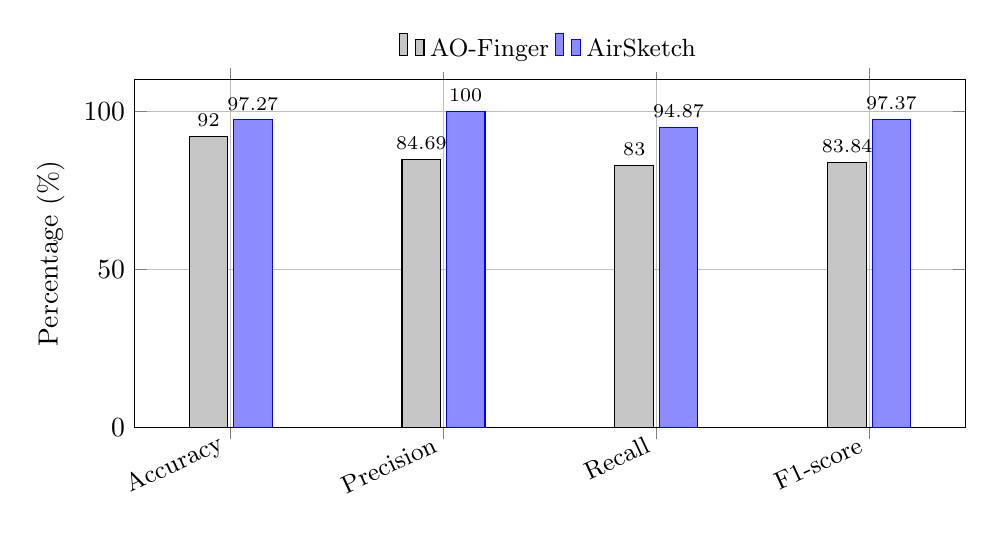
\begin{tikzpicture}
\begin{axis}[
    ybar,
    bar width=14pt,
    width=\columnwidth,
    height=6cm,
    ymin=0,
    ymax=110,
    ylabel={Percentage (\%)},
    symbolic x coords={Accuracy,Precision,Recall,F1-score},
    xtick=data,
    x tick label style={
        rotate=25,
        anchor=east,
        font=\small
    },
    nodes near coords,
    nodes near coords align={vertical},
    nodes near coords style={font=\scriptsize},
    enlarge x limits=0.15,
    grid=major,
    legend style={
        at={(0.5,1.02)},
        anchor=south,
        legend columns=2,
        font=\small,
        draw=none
    },
    legend cell align=left
]

% AO-Finger (Left Bar)
\addplot[
    fill=gray!45,
    draw=black
] coordinates {
    (Accuracy,92.00)
    (Precision,84.69)
    (Recall,83.00)
    (F1-score,83.84)
};

% AirSketch (Right Bar)
\addplot[
    fill=blue!45,
    draw=blue
] coordinates {
    (Accuracy,97.27)
    (Precision,100.00)
    (Recall,94.87)
    (F1-score,97.37)
};

\legend{AO-Finger,AirSketch}

\end{axis}
\end{tikzpicture}
\caption{Comparative evaluation of AO-Finger and AirSketch
for binary pinch detection. AO-Finger metrics are derived
from its published confusion matrix.}
\label{fig:metrics}
\end{figure}


The quantitative evaluation indicates that the current pinch detector performs consistently on the available evaluation samples. The measured accuracy of 97.27\% indicates that 285 of the 293 labeled samples were classified correctly. More specifically, all 137 no-pinch samples in the evaluation were correctly identified, while 148 of the 156 actual pinch samples were correctly detected.

The precision of 100.00\% is particularly relevant to the interaction design because no sampled no-pinch frame was incorrectly interpreted as a pinch. In the context of AirSketch, a false-positive pinch could unintentionally activate drawing or a shape operation. The observed zero false-positive rate therefore indicates that such an error did not occur in the available evaluation samples.

The recall of 94.87\% shows that the detector did not identify every actual pinch sample. The eight false-negative samples account for the complete set of observed errors. This suggests that future threshold adaptation or temporal gesture stabilization could focus on reducing missed pinch states without unnecessarily increasing false-positive activations.


AO-Finger reported a pinch precision of 83\% in its sample-level evaluation, whereas AirSketch achieved 100\% pinch precision on its available evaluation samples \cite{ao_finger}.

AO-Finger uses dedicated acoustic-optic wrist-worn sensing hardware, while AirSketch uses a standard RGB webcam and MediaPipe landmarks. The datasets, participants, gesture definitions, sampling procedures, and evaluation protocols are also different.

The comparison is therefore limited to the reported pinch-precision values under their respective evaluation conditions. Within the AirSketch evaluation, no false-positive pinch predictions were observed. This demonstrates that a webcam-based landmark approach can provide high pinch-detection precision for the specific virtual drawing interaction implemented in AirSketch, without requiring dedicated acoustic-optic sensing hardware.

The comparison also highlights the different objectives of the two systems. AO-Finger is designed for fine-grained finger gesture recognition using multimodal wearable sensing, while AirSketch is designed as a lightweight application-level drawing interface. AirSketch therefore does not attempt to reproduce the broader sensing capabilities of AO-Finger.

\subsection{Novelty}
The primary novelty of AirSketch is not a new hand-landmark detector or a new machine-learning architecture. Instead, the contribution lies in integrating established hand landmark detection with a deterministic interaction model for a complete virtual drawing application.

This application-level integration makes the system comparatively simple to inspect and modify. The gesture logic does not depend on a project-specific trained classifier, which also reduces the need for a dedicated gesture dataset for the basic interaction vocabulary.

\section{Future Improvements}
Several limitations remain in the current implementation. The system supports only single-hand tracking, restricting two-handed interactions, and relies on a fixed 1280 × 720 coordinate space, which limits adaptability to different camera configurations. Additionally, the pinch detection mechanism uses a fixed pixel threshold, making it sensitive to variations in hand size and camera distance. Future versions could address these limitations through multi-hand tracking, dynamic frame dimensions, and normalized distance thresholds.

The system currently relies on geometric landmark-based rules rather than a learned gesture classifier. While this approach offers simplicity and interpretability, it limits the range of supported gestures. Future work could explore lightweight classification models and temporal deep-learning techniques for recognizing additional static and dynamic gestures \cite{moreira2026,anithadevi2025}, while retaining deterministic rules for core drawing operations.


\section{Conclusion}

This paper presented AirSketch, a real-time webcam-based virtual drawing and control system implemented using Python, OpenCV, MediaPipe, and NumPy. The system uses MediaPipe's 21-point hand representation to obtain fingertip coordinates, uses the index fingertip as a virtual pointer, and determines the primary interaction state using the Euclidean distance between the index and middle fingertips.

A frame-level evaluation using 293 labeled samples produced 97.27\% accuracy, 100.00\% precision, 94.87\% recall, and 97.37\% F1-score. The confusion matrix contained 148 true positives, 137 true negatives, zero false positives, and eight false negatives. The observed errors were therefore exclusively false negatives in the available evaluation set.

A comparison with AO-Finger showed that AirSketch achieved higher reported pinch precision under its own evaluation conditions than the 83\% pinch precision reported by AO-Finger.

Overall, AirSketch demonstrates that a standard webcam combined with MediaPipe landmarks and deterministic geometric interaction rules can support a practical virtual drawing interface without specialized wearable sensing hardware. The system provides a lightweight foundation for future work involving adaptive gesture thresholds, multi-hand interaction, richer gesture vocabularies, and more extensive user-centered evaluation.

\begin{thebibliography}{00}

\bibitem{ao_finger}
C. Xu, B. Zhou, G. Krishnan, and S. Nayar,
``AO-Finger: Hands-free Fine-grained Finger Gesture Recognition via Acoustic-Optic Sensor Fusing,''
in \emph{Proc. CHI Conference on Human Factors in Computing Systems (CHI)}, 2023,
doi: 10.1145/3544548.3581264.

\bibitem{omgbench}
H. Chang, P. Ren, B. Zhang, D. Li, T. Han, H. Zhang, L. Xie,
H. Chen, and E. Yin,
``OMG-Bench: A New Challenging Benchmark for Skeleton-based Online Micro Hand Gesture Recognition,''
2026.

\bibitem{airwriting}
H. Jand and S. Ranjan,
``Air Writing App with Real-Time Hand Tracking and Handwriting Recognition using Fingertip Detection and Drawing,''
\emph{International Journal on Recent and Innovation Trends in Computing and Communication},
vol. 11, no. 10, pp. 1147--1153, 2023.

\bibitem{swathi}
S. A. Swathi,
``Air Canvas Hand Tracking,''
\emph{Journal of Emerging Technologies and Innovative Research},
vol. 11, no. 11, 2024.

\bibitem{mahmud}
H. Mahmud, M. M. Morshed, and Md. Kamrul Hasan,
``A Deep Learning-based Multimodal Depth-Aware Dynamic Hand Gesture Recognition System,''
2021.

\bibitem{sharma}
A. Sharma, A. Mittal, S. Singh, and V. Awatramani,
``Hand Gesture Recognition using Image Processing and Feature Extraction Techniques,''
\emph{Procedia Computer Science},
vol. 173, pp. 181--190, 2020,
doi: 10.1016/j.procs.2020.06.022.

\bibitem{qi2024}
J. Qi, L. Ma, Z. Cui, and Y. Yu,
``Computer vision-based hand gesture recognition for human-robot interaction: a review,''
\emph{Complex \& Intelligent Systems},
vol. 10, pp. 1581--1606, 2024,
doi: 10.1007/s40747-023-01173-6.

\bibitem{morajkar}
A. Morajkar, A. M. James, M. Bagwe, A. S. James, and A. Pavate,
``Hand gesture and voice-controlled mouse for physically challenged using computer vision,''
\emph{Advanced Engineering Days},
vol. 6, pp. 127--131, 2023.

\bibitem{anithadevi2025}
N. Anithadevi, S. Palanisamy, S. S. Rubini, and S. Shrestha,
``MediaPipe-LSTM-Enhanced Framework for Real-Time Dynamic Sign Language Recognition in Inclusive Communication Systems,''
\emph{Engineering Reports}, 2025.

\bibitem{quan}
L. Quan, Q. Guo, X. Xie, S. Chen, X. Li, and Y. Liu,
``Towards Understanding the Faults of JavaScript-Based Deep Learning Systems,''
in \emph{Proc. IEEE/ACM International Conference on Automated Software Engineering (ASE)}, 2022,
doi: 10.1145/3551349.3560427.

\bibitem{vasavi}
R. Vasavi, N. Rahul, A. Snigdha, K. J. Moses, and S. V. Simha,
``Painting with Hand Gestures using MediaPipe,''
\emph{International Journal of Innovative Science and Research Technology},
vol. 7, no. 12, 2022.

\bibitem{moreira2026}
J. Moreira,
``Dynamic LIBRAS Gesture Recognition via CNN over Spatiotemporal Matrix Representation,''
arXiv:2603.25863, 2026.

\bibitem{generative_airsketch}
H. X. G. Lim, X. Cui, Y. S. Rawat, and S.-N. Lim,
``AirSketch: Generative Motion to Sketch,''
in \emph{Advances in Neural Information Processing Systems (NeurIPS)}, 2024,
arXiv:2407.08906.

\bibitem{virtualwrite}
S. Barade, P. Kadam, P. Vedpathak, and N. S. Bahirame,
``Virtual Write and Clear Application: A Gesture-based Drawing Tool using Mediapipe and OpenCV,''
\emph{International Journal for Multidisciplinary Research in Science, Engineering and Technology},
vol. 8, no. 3, 2025,
doi: 10.15680/IJMRSET.2025.0803129.

\bibitem{virtualpainting}
S. V. Tiwari, D. A. Vartak, V. R. Verma, A. I. Sayyed, and S. Khatu,
``Virtual Hand Gesture Painting,''
2024.

\bibitem{repo}
Code-Hish, ``MajorProject: New\_Airsketch\_Codes,'' GitHub repository, 2026. [Online]. Available: \url{https://github.com/Code-Hish/MajorProject/tree/main/New_Airsketch_Codes}

\end{thebibliography}

\end{document}

\end{document}
